Exponer los resultados obtenidos, utilizando para esto el apoyo de tablas, figuras, entre otros.

Un ejemplo de una tabla se presenta en Tabla \ref{C1T1:tableExample}
%%%---------- Table C3T1. tableExample ----------%%%
%%\input{../03Tables/01Chapter/C1T1:tableExample}

%%%---------- Table C1T1. tableExample ----------%%%
%\input{03Tables/01Chapter/C1T1:tableExample}

\begin{table}[H]
    \caption{Table Example.\label{C1T1:tableExample}}
    \newcolumntype{C}{>{\centering\arraybackslash}X}
        \begin{tabularx}{\textwidth}{CCCC}
            \toprule
            \textbf{TITLE 1} & \textbf{TITLE 2}   & \textbf{TITLE 3} & \textbf{TITLE 4}        \\
            \midrule
            TEXT 1   & TEXT 2 & TEXT 3 & TEXT 4 \\
            …        & …     & …    & …     \\  
            TEXT n   & TEXT n & TEXT n & TEXT N \\
            \bottomrule
        \end{tabularx}
\end{table}

Un ejemplo de una figura se presenta en Figura \ref{C1F1:figureExample}
%%%---------- Figure C3F1. figureExample ----------%%%
\begin{figure}[H]
    \centering
    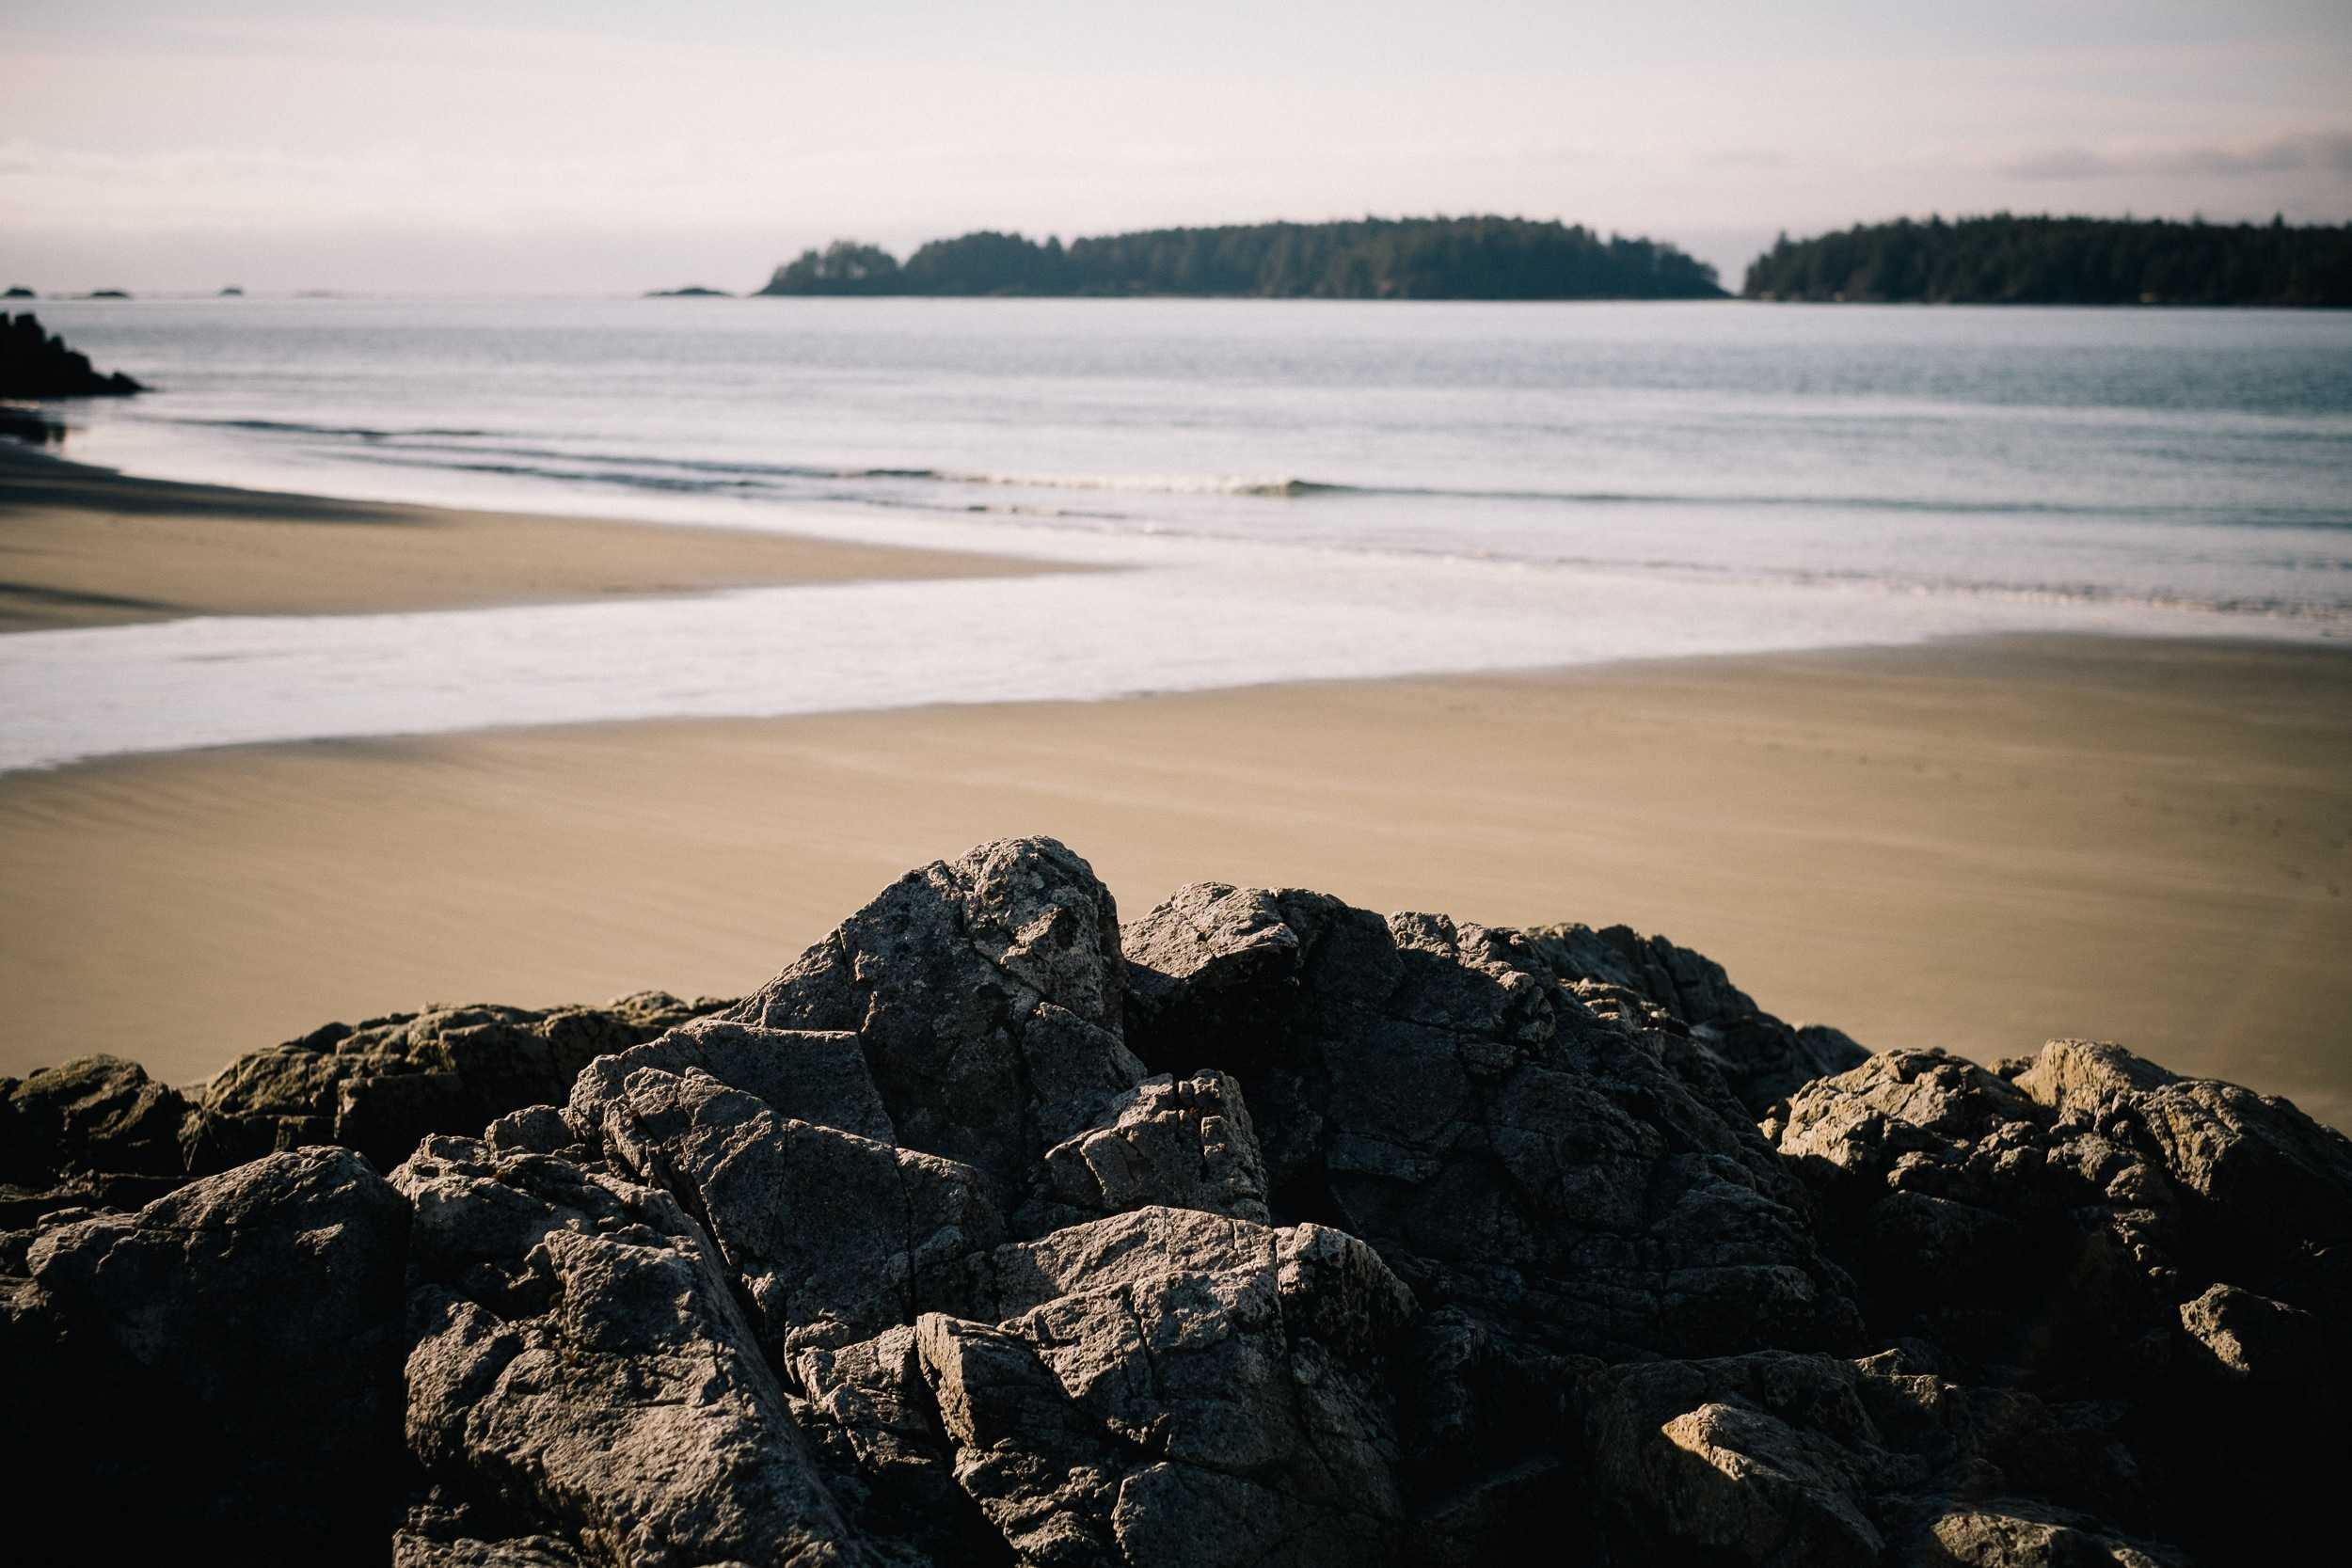
\includegraphics[width=0.8\textwidth]{../02Figures/01Chapter/C1F1_figureExample.png}
    \caption{Figure Example}
    \label{C1F1:figureExample}
\end{figure}

Un ejemplo de una ecuación se presenta en Ecuación \ref{C3E1:equiationExample}
%%%---------- Equation C3E1. equationExample ----------%%%
\begin{equation}\label{C3E1:equiationExample}
    (x+y)^2 = x^2 + 2 \cdot x \cdot y + y^2
\end{equation}
    